%%%%% PREAMBLE %%%%%
\documentclass{article}

% american mathematical society
\usepackage{amsmath,amsthm,amssymb}
% allow align enviroment to be split on multiple pages
\allowdisplaybreaks

    % definition of theorem enviroments and numbering scheme 
    \newtheorem{theorem}{Theorem}[section]
    \newtheorem{proposition}[theorem]{Proposition}

    \theoremstyle{definition}
    \newtheorem{definition}[theorem]{Definition}
    \newtheorem{problem}[theorem]{Problem}

    % equation numbering
    \numberwithin{equation}{section}

    % math operators
    \DeclareMathOperator*{\argmin}{argmin}
    \DeclareMathOperator*{\var}{Var}
    \DeclareMathOperator*{\cov}{Cov}
    \DeclareMathOperator{\VaR}{VaR}
    \DeclareMathOperator{\cvar}{CVaR}

% additional math font types
\usepackage{mathrsfs}

% add functionality to enumerate enviroment
\usepackage{enumitem}

%%% COMMENT COMMAND %%%
% load required package
\usepackage[dvipsnames]{xcolor}
% definition of comment color
\newcommand{\commentcolor}{Goldenrod}
\newcommand{\taskcolor}{RedOrange}
% definition of comment function itself
\newcommand{\comment}[1]{
    \begin{center}
        \colorbox{\commentcolor}{
            \textsf{
                \textbf{#1}
            }
        }
    \end{center}
}
\newcommand{\task}[1]{
    \begin{center}
        \colorbox{\taskcolor}{
            \textsf{
                \textbf{#1}
            }
        }
    \end{center}
}
                        
% drawing functionality
\usepackage{tikz}
\usetikzlibrary{matrix}

% automatically include a float barrier in sections
\usepackage[section]{placeins}

% reference name
\usepackage{nameref}

% clickable references
\usepackage[hidelinks]{hyperref}

%%%%% MAIN DOCUMENT %%%%%
\begin{document}

\begin{titlepage}
    \begin{center}
        {\huge\textbf{Financial Engineering}}\\[2mm]
        {\Large Kasper Rosenkrands}\\[2cm]
        {\large MATØK6}\\[2mm]
        {\large Spring 2020}
    \end{center}
    
    \vfill
\end{titlepage}

\section{Bonds and the Value of Money Through Time}
\textit{Here you can explain what type of interests we studied and how the fair-price of bonds depends on these types of interest and viceversa.}

\subsection{Bonds}
I will begin by giving the definition of a bond.
\begin{definition}[Bond]
    A bond is a financial security that pays the owner a chain of predetermined payments.\label{def:bond}
\end{definition}
Using definition \ref{def:bond} we can interpret a bond as a financial asset which have no risk.
In order words we know for a fact how much money we will make on this investment, disregarding the inherent risk of default.

\subsection{Value of Money Through Time}
The value of money changes through time.
Assume you were offered an amount of money with value $M$, furthermore you would have the choice of recieving the money today or 1 year from now.
Choosing to recieve the money now you would be able to spend them straightaway which could be preferable compared to waiting a year.
Prices could also have risen during the waiting time, further diminishing the value.
Last but not least, recieving the money today would enable you to put the money in the bank and thereby recieve a premium.
All these arguments serve the purpose of showing that the value of money changes through time, and that the value $M$ of the money would decrease by waiting a year before recieving the money.

\subsection{Interest Rate}
The premium recieved by depositing money at bank mentioned earlier is described by an interest rate.
This interest rate will in the following be described by a positive number $$r>0.$$
Different types of interest exists and i will describe the following three types
\begin{enumerate}
    \item simple interest,
    \item compouned interest,
    \item continuously compounded interes.
\end{enumerate}
Common for all three types is that they represent a fraction of an investment that is paid either ones or through several periods.

However to further dive into the different types of interest we will first define the notion of a wealth process.
\begin{definition}[Wealth Process]
    The evolution of an investment over time is called the wealth process of that investment and is denoted by
    \begin{align}
        V = (V_t)_{0 \leq t \leq T}.
    \end{align}
    The initial capital is denoted by $v_0$, and we assume that $V$ is a real-valued stochastic process on a given probability space $(\Omega, \mathscr{F}, \mathbb{P})$.
\end{definition}
With this definition in place we are now ready to define the three different types of interest starting with simple interest.
\begin{definition}[Simple Interest]
    Let $v_0 \in \mathbb{R}$ be our initial capital.
    An interest on $v_0$ is said to be simple if it follows the wealth process
    \begin{align}\label{eq:simple_interest_wealth_process}
        V_t = (1 + rt)v_0, \quad 0 \leq t \leq T.
    \end{align}
\end{definition}
I will now show that the wealth process in \eqref{eq:simple_interest_wealth_process} is indeed a stochastic process in any probability space.
Any stochastic process $X$ on the probability space $(\Omega, \mathscr{F}, \mathbb{P})$ satisfies
\begin{align}
    \{\omega \in \Omega \, : \, X(\omega) \leq x\} \in \mathscr{F}, \quad \forall x \in \mathbb{R}.
\end{align}
Suppose $v_0 > 0$ and $x \geq (1 + rt)v_0$ then
\begin{align}
    \{\omega \in \Omega \, : \, (1 + rt)v_0 \leq x\} = \{\Omega\} \in \mathscr{F},
\end{align}
on the other hand if $x < (1 + rt)v_0$
\begin{align}
    \{\omega \in \Omega \, : \, (1 + rt)v_0 \leq x\} = \{\emptyset\} \in \mathscr{F}.
\end{align}
As both $\Omega$ and $\emptyset$ is contained in any $\sigma$-algebra we have shown that the wealth process in \eqref{eq:simple_interest_wealth_process} is a stochastic process in any probability space.
Next i will define the notion of compund interest.
\begin{definition}[Compounded Interest]
    Let $v_0 \in \mathbb{R}$ be our initial capital.
    An interest on $v_0$ is said to be compunded over $m\in\mathbb{N}$ periods if it follows the wealth process
    \begin{align}\label{eq:compund_interest_wealth_process}
        V_t = \left( 1 + \frac{r}{m} \right)^{mt} v_0, \quad 0 \leq t \leq T.
    \end{align}
\end{definition}
As stated in the definition $m$ can be any natural number, however if $m = 1, 12, 365$ the interest is refered to as annually, monthly and daily compounded, respectively.
Note that we have the following properties $\forall\, 0 \leq t \leq T$
\begin{enumerate}[label = \textit{\roman*})]
    \item $V_{t + 1} = \left( 1 + \dfrac{r}{m} \right)^{m}V_t$,
    \item If $m_1 > m_2, v_0 > 0 
    \, \Rightarrow \, 
    \left( 1 + \dfrac{r}{m_1} \right)^{m_1t}v_0
    >
    \left( 1 + \dfrac{r}{m_2} \right)^{m_2t}v_0$,
    \item If $m_1 > m_2, v_0 < 0 
    \, \Rightarrow \, 
    \left( 1 + \dfrac{r}{m_1} \right)^{m_1t}v_0
    <
    \left( 1 + \dfrac{r}{m_2} \right)^{m_2t}v_0$.
\end{enumerate}
From this is follows that for an \textit{investor} compund interest is more attractive as it pays more, however as a \textit{debtor} it is less attractive as he or she will have to pay more on his or hers debt.

At last i can turn to continuously compounded interest which i will present as the limit of \eqref{eq:compund_interest_wealth_process} as $m \rightarrow \infty$.
Note that by the following definition of $e$
\begin{align}
    \lim_{x \rightarrow \infty} \left(1 + \frac{1}{x}\right)^x = e,
\end{align}
by letting $x = r/m$ in the above the limit of the wealth process of compounded interest can be seen as
\begin{align}
    \left[\left( 1 + \frac{r}{m} \right)^\frac{m}{r}\right]^{rt}v_0 \rightarrow
    (e)^{rt}v_0, \quad \text{as } m \rightarrow \infty.
\end{align} 
This leads to the definition of continuously compounded interest.
\begin{definition}[Continuously Compounded Interest]
    Let $v_0$ be our initial capital.
    An interest on $v_0$ is said to be continuously compounded at rate $r>0$ if the wealth process
    \begin{align}
        V_t = e^{rt}v_0, \quad 0 \leq t \leq T.
    \end{align}
\end{definition}
There exists the following relation between the different types of interest
\begin{align}
    (1 + r) \leq \left(1 + \frac{r}{m}\right)^m < e^r.
\end{align}
To show that the relation indeed holds i will show that the sequence
\begin{align}
    a_m = \left(1 + \frac{r}{m}\right)^m,
\end{align}
is increasing.

Using the binomial theorem
\begin{align*}
    (x+y)^n = \sum_{k=0}^n \begin{pmatrix} n \\ k \end{pmatrix} x^k y^{n-k}
\end{align*}
we have 
\begin{align*}
    \left( 1 + \frac{r}{m} \right)^m &= \sum_{k=0}^m \begin{pmatrix} m \\ k \end{pmatrix} 1^{m-k}\begin{pmatrix} \frac{r}{m} \end{pmatrix}^k\\
    &= \sum_{k=0}^m \begin{pmatrix} m \\ k \end{pmatrix} \begin{pmatrix} \frac{r}{m} \end{pmatrix}^k := \clubsuit
\end{align*}
Each term is of the form
\begin{align*}
    \begin{pmatrix} m \\ k \end{pmatrix}\begin{pmatrix} \frac{r}{m} \end{pmatrix}^k = \prod_{l=0}^{k-1} \frac{m-l}{k + l} \begin{pmatrix} \frac{r}{m} \end{pmatrix}
\end{align*}
Each term is of the form
\begin{align*}
    \frac{m-l}{k+l} \frac{r}{m} &= \frac{rm - lr}{m(k+l)}\\
    &= \frac{m(r - lr/m)}{m(k+1)}\\
    &= \frac{r - lr/m}{k+l} := \bigstar
\end{align*}
The term $\bigstar$ increases with $m$ and thus the product increases with $m$ and thus the sum $\clubsuit$ increases with $m$ and therefore it is an increasing sequence. 

\subsection{Types of Bonds}
A bond is a financial security that pays to the owner, a chain of predetermined payments.
However there are different types of bonds.
I will discuss the following two types here
\begin{enumerate}
    \item zero-coupon bonds,
    \item coupon bonds.
\end{enumerate}
A \textbf{zero-coupon bond} is a bond with a single payment $F > 0$ at time $T > 0$.
The pay-off F is called the face value and $T$ the maturity time.
The next question i will answer is how much i will be willing to pay for such a financial assest.
This depends on the way the time value of money is measured.
Consider for example the following setup; let $B_0 \geq 0$ be the value of the zero-coupon bond with face value $F>0$ and maturity time $T>0$.
Suppose that only annual compound interest at rate $r>0$ is available.
From a buyers perspective what if
\begin{align}\label{eq:zero_coupon_bond_example}
    B_0 > \frac{F}{(1 + r)^T},
\end{align}
would i buy the bond? 
No, of course not because the right side of \eqref{eq:zero_coupon_bond_example} denote the amount of money i would have to put in the bank today to recieve exactly $F$ at time $T$.
When the aforementioned amount of monwy is less than the price of the bond, i would surely choose to put money in the bank instead of buying the bond, as the bond will pays exactly $F$ at time $T$.
Suppose now that we flip the inequality and look from a sellers perspective, that is if
\begin{align}\label{eq:zero_coupon_bond_example_seller}
    B_0 < \frac{F}{(1 + r)^T},
\end{align}
would i sell the bond? 
No of course not because the right side of \eqref{eq:zero_coupon_bond_example_seller} denotes the amount at i can borrow at time 0 if i agree to pay exactly $F$ at time $T$.
For the bond i would also have to pay $F$ at time zero however i would only recieve $B_0$ at time 0.
Therefore i would not agree to sell the bond in this situation.

This implies that the only price a buyer and seller can agree to is in the situation where
\begin{align}
    B_0 = \frac{F}{(1 + r)^T}.
\end{align}
Now i will consider the situatuion where at time $1 \leq t \leq T$ i want to get rid of a bond, but i what to determine what price i should sell it to.
At this time the bond can be considered a new zero-coupon bond with face value $F > 0$ and maturity time $T - t$.
Thus we have from the previous argumentation that
\begin{align}
    B_t = \frac{F}{(1 + r)^{T - t}}, \quad 0 \leq t \leq T.
\end{align} 

The chain of arguments holds also when the time value of money is different, if a compounded interest over $m$ periods where considered then the fair price of a zero-coupon bond at time $t$ would be
\begin{align}
    B_t = \frac{F}{\left(1 + \frac{r}{m}\right)^{m(T - t)}}.
\end{align}
If we consider the continuously compounded case the fair price would be
\begin{align}
    B_t = \frac{F}{e^{r(T -t)}}.
\end{align}

A \textbf{coupon bond} guarantees the owner a payment $F > 0$ at time $T > 0$, as well as a fixed amount $C > 0$ at $t = 1,2,\ldots,T$.
To find a fair price for such a bond i will follow the same argumentation as above, namely i will compare the price of the bond with the cost of recieving the same benefits with a bank account.
In other words how much money will i have to deposit in my bank account today if i want to
\begin{align}
    \text{1.} \quad &\text{withdraw $C > 0$ after 1 year} \\
    \text{2.} \quad &\text{withdraw $C > 0$ after 2 years} \\
    &\quad \vdots \\
    \text{$T-1$.} \quad &\text{withdraw $C > 0$ after $T-1$ years} \\
    \text{$T$.} \quad &\text{withdraw $F + C$ after $T$ years}
\end{align}
and have nothing left in the bank account afterwards.

In order to be able to get $C > 0$ after one year i have to put
\begin{align}
    \frac{C}{1+r}
\end{align}
in the bank.
In order to be able to get $C > 0$ after two years i have to put 
\begin{align}
    \frac{C}{(1+r)^2}
\end{align}
in the bank.
Generalizing this argument tells me that in order to recieve $C > 0$ after $t$ years i have to put
\begin{align}
    \frac{C}{(1+r)^t}
\end{align}
in the bank.
Lastly in order to get $F + C$ after $T$ years i have to put
\begin{align}
    \frac{F + C}{(1+r)^T} = \frac{F}{(1+r)^T} + \frac{C}{(1+r)^T}
\end{align}
in the bank.
Adding up all these amounts it is concluded that i have to make a deposit of
\begin{align}
    \sum_{i = 1}^T \frac{C}{(1 + r)^i} + \frac{F}{(1+r)^T}.
\end{align}
The agreeable price of a coupon bond is thus given by
\begin{align}
    B_0 = 
    \sum_{i = 1}^T \frac{C}{(1 + r)^i} + \frac{F}{(1+r)^T} =
    \frac{\xi_T}{(1 + r)^T}.
\end{align}
Where the pay-off $\xi_T$ at time $T$ is given by
\begin{align}
    \xi_T := \sum_{i = 1}^T C(1 + r)^{T -i} + F,
\end{align}
in other words the fair price of the coupon bond (as well as the zero-coupon bond) can be written as the discounted price of the total pay-off.
\newpage

\section{Portfolio Allocation and Risk Measures}
\textit{Try to explain what a portfolio is and how we can create (allocate) portfolio based on risk measures. In your discussion about the latter, remember to include the differences/benefits/drawbacks of considering the standard deviation, VaR and CVaR as risk measures.}

\subsection{Portfolio}
First and foremost i will give the definition of a portfolio.

\begin{definition}[Portfolio and Strategies]
    Let
    \begin{align}
        \mathfrak{M} = \left\{ 
            \left(
                \Omega, \mathscr{F}, \mathbb{P}
            \right),
            P = \left(
                B_t, S_t^{(1)}, \ldots, S_t^{(d)}
            \right)_{0 \leq t \leq T}
         \right\},
    \end{align}
    be a finite-horizon financial market.
    A portfolio in $\mathfrak{M}$ is a $(d + 1)$-dimensional vector
    \begin{align}
        \Theta_t = \left(\varphi_t, \theta_t^{(1)}, \ldots, \theta_t^{(d)}\right),
    \end{align}
    in which
    \begin{align}
        \Theta_t^j = \text{Number of shares of the $j$'th asset held between time $t-1$ and $t$}.
    \end{align}
    for $j = 1, \ldots, d + 1$.
    The collection $\Theta = \left( \Theta_t \right)_{0 \leq t \leq T}$, with the convention that $\Theta_0 = \Theta_1$, is termed a strategy.
\end{definition}
For every strategy on market there is an associated wealth process.
The wealth process for $\Theta$ is defined and denoted by
\begin{align}
    V_t^{\Theta} = \varphi_t B_t + \sum_{j = 1}^d \theta_t^{(j)} S_t^{(j)} = \Theta_t \cdot P_t, \quad 0 \leq t \leq T.    
\end{align}

\subsection{Risk Measures}
Any strategy on a given market inherently carries a risk because the return is random, there is in other words no way to predict our profit or losses with certainty.
There is no one way to measure the risk associated with a strategy, however in the next two sections i will explore two approaches.
Both of these is based on portfolio allocation as an optimization problem.
The problem is given in this way; solve
\begin{align}
    \argmin_{\mathbf{w}\in\mathbb{R}^{d+1}}
    \mathcal{R}\left( \mathbf{w} \cdot \mathbf{K}_P \right),
\end{align}
subject to:
\begin{align}
    \sum_{j = 0}^d w_j = 1, \ 
    \mathbb{E}\left[ U(\mathbf{w} \cdot \mathbf{K}_P) \right] = \mu, \
    \mu \in \mathbb{R},
\end{align}
where $\mathcal{R}$ is a measure of risk and $U(\mathbf{w} \cdot \mathbf{K}_P)$ is the utility of the strategy.

\subsubsection{Mean-Variance}
If an agent would like to maximize profit while minimizing the variance, he or she could take the mean-variance approach.
In this approach risk is measured using standard deviations, i.e.
\begin{align}
    \mathcal{R}(X) = \sigma(X) = \sqrt{\var(X)} = \sqrt{\mathbb{E}\left[ (X - \mathbb{E}(X))^2 \right]}.
\end{align}
For a portfolio with weights $\mathbf{w}$, we have that
\begin{align}
    \mathcal{R}(\mathbf{w} \cdot \mathbf{K}_P) = \sqrt{\mathbf{w}^\top C \mathbf{w}},
\end{align}
where $C$ is a $(d + 1) \times (d + 1)$ matrix given by
\begin{align}
    C^{i,j} = 
    \cov\left( \mathbf{K}_P^i, \mathbf{K}_P^j \right) =
    \sqrt{\mathbb{E}\left[ \left( \mathbf{K}_P^i - \mathbb{E}(\mathbf{K}_P^i) \right) \left( \mathbf{K}_P^j - \mathbb{E}(\mathbf{K}_P^j) \right) \right]}.
\end{align}
\comment{Write exercise from lecture 2}
The mean variance approach assumes the uitility function as the identity, that is
\begin{align}
    U(x) = x.
\end{align}
By letting
\begin{align}
    \mu_\mathbf{K} := \mathbb{E}\left[\mathbf{K}_P\right],
\end{align}
it follows that
\begin{align}
    \mathbb{E}\left[ U(\mathbf{w} \cdot \mathbf{K}_P) \right] = \mathbf{w} \cdot \mu_\mathbf{K}.
\end{align}
Thus the optimization problem, in the mean-variance approach becomes
\begin{problem}[Optimization Problem Mean-Variance]
    \begin{align}
        &\quad\argmin_{\mathbf{w}\in\mathbb{R}^{d+1}} \sqrt{\mathbf{w}^\top C \mathbf{w}} \\
        &\text{Subject to:} \nonumber \\
        &\qquad \text{1.) }\sum_{j = 0}^d w_j = 1, \\
        &\qquad \text{2.) }\mathbf{w} \cdot \mu_\mathbf{K} = \mu, \quad \mu \in \mathbb{R}.
    \end{align}
\end{problem}
An illustrative example to demonstrate why one might consider a different risk measure than the standard deviation is the following.
Consider two portfolios that generate the following wealth
\begin{align}
    V_1^{(1)} = 
    \begin{cases}
        1 &\text{with probability $1/2$} \\
        -9 &\text{with probability $1/2$}    
    \end{cases}
\end{align}
and
\begin{align}
    V_1^{(2)} = 
    \begin{cases}
        5 &\text{with probability $1/2$} \\
        -5 &\text{with probability $1/2$}    
    \end{cases}
\end{align}
According to their standard deviation these two portfolios carries the same risk, but one could argue that the first is riskier that the latter.
The next risk measure i will consider i concerned with controlling losses rather than the variation of the return.

\subsubsection{Value at Risk}
If i denote the outcome of an investment with $V_1$ then our potential losses will be given by $-V_1$.
Suppose that for some $x \in \mathbb{R}$
\begin{align}
    -V_1 \leq x.
\end{align}
Then to cover my risk of bankruptcy i must keep at least the amount $x$ in my bank account.
In reality the only thing i can quantify is the chance of the happening, which is denoted by
\begin{align}
    \mathbb{P}\left( -V_1 \leq x \right).
\end{align}
This is the motivation behind the risk measure value at risk.
\begin{definition}[Value at Risk]
    Let $0 < \alpha < 1$ and $X$ be a random variable.
    The Value at Risk (VaR) of $X$ is defined and denoted by
    \begin{align}
        \VaR_\alpha(X) := \inf
        \left\{
            x \in \mathbb{R} \, : \,
            \mathbb{P}(X + x \geq 0)
            \geq 1 - \alpha
        \right\}.
    \end{align}
\end{definition}
In other words the $\VaR_\alpha(X)$ represents the amount of extra capital i need to hold in order to reduce my risk of bankruptcy to $1 - \alpha$.
An alternative representation of $\VaR$ can be formulated using the fact that
\begin{align}
    \mathbb{P}(-X \leq x) \geq 1 - \alpha
    \, \Longleftrightarrow \,
    \mathbb{P}(X + x < 0) \leq \alpha,
\end{align}
this lets us formulate an equivalent representation given by
\begin{align}
    \VaR_\alpha(X) := \inf
    \left\{
        x \in \mathbb{R} \, : \,
        \mathbb{P}(X < -x) \leq \alpha
    \right\}.
\end{align}
The following proposition describes some properties for the $\VaR$.
\begin{proposition}[Properties of $\VaR$]
    Let $X, Y$ be arbitrary random variables.
    Then, the following holds
    \begin{enumerate}
        \item If $X \geq 0$ almost surely, then $\VaR_\alpha(X) \leq 0$.
        \item For all $y\in \mathbb{R}$ we have that $\VaR_\alpha(X + y) = \VaR_\alpha(X) - y$. In particular $\VaR_\alpha(X + \VaR_\alpha(X)) = 0$.
        \item If $\lambda \geq 0$, then $\VaR_\alpha(\lambda X) = \lambda \VaR_\alpha(X)$.
        \item If $X \geq Y$ almost surely, then $\VaR_\alpha(X) \leq \VaR_\alpha(Y)$.
    \end{enumerate}
\end{proposition}
\begin{proof}
    \comment{Get back to this proof}
\end{proof}

\subsection{Coherent Risk Measures}

There are one important drawback to measuring risk using $\VaR$ and that is its lack of diversification.

Note that when using the standard deviation as a risk measure we get the following
\begin{align}
    \sigma(X + Y)^2 = \var(X) + \var(Y) + 2\rho_{X,Y}\sqrt{\var(X)\var(Y)},
\end{align}
where $\rho_{X,Y} = \frac{\cov(X,Y)}{\sqrt{\var(X)\var(Y)}} \leq 1$.
Then
\begin{align}
    \sigma(X + Y)^2 &= \sigma(X)^2 + \sigma(Y)^2 + 2\rho_{X,Y}\sigma(X)\sigma(Y)\\
    &\leq \sigma(X)^2 + \sigma(Y)^2 + 2\sigma(Y)\sigma(X) = \left[\sigma(X) + \sigma(Y)\right]^2, 
\end{align}
which would imply that
\begin{align}
    \sigma(X + Y) \leq \sigma(X) + \sigma(Y).
\end{align}
This means that, under the risk measure $\sigma$, investing in $X + Y$ carries less risk than investing in $X$ or $Y$ seperately.
The phenomenon is better known as diversification, and it is common belief that diversification of a portfolio lowers the risk.
However $\VaR$ as a risk measure is not able to reproduce this, that is in general we do not have that
\begin{align}
    \VaR_\alpha(X + Y) \leq \VaR_\alpha(X) + \VaR_\alpha(Y).
\end{align}
As diversification is a desired i will know introduce the concept of Coherent Risk Measures.

Fix a probability space $(\Omega, \mathscr{F}, \mathbb{P})$, i will use the following notation
\begin{align}
    L^p = \{X \, : \, \Omega \rightarrow \mathbb{R} \, : \, X \text{ r.v. such that } \mathbb{E}(|X|^p) < \infty\}.
\end{align}
I will now give the definition
\begin{definition}[Coherent Risk Measure]
    A function $\rho \, : \, L^1 \rightarrow \mathbb{R}$ is said to be a Coherent Risk Measure if
    \begin{enumerate}
        \item If $X \geq 0$ almost surely, then $\rho(X) \leq 0$.
        \item For all $y \in \mathbb{R}$ we have that $\rho(X + y) = \rho(X) - y$.
        \item If $\lambda \geq 0$, then $\rho(\lambda X) = \lambda \rho(X)$.
        \item We have that $\rho(X + Y) \leq \rho(X) + \rho(Y)$.
    \end{enumerate}
\end{definition}

\subsubsection{Conditional Value at Risk}
The Conditional Value at Risk (CVAR) is a common example of a coherent risk measure.
This section will explore this particular risk measure further.

Given a random variable $X$, we will write
\begin{align}
    q_\alpha(X) := \inf \{x \, : \, \mathbb{P}(X \leq x) \geq \alpha\}.
\end{align}
With this notation now introduced i can present the definition of CVaR
\begin{definition}[Condition Value at Risk]
    Let $ 0 < \alpha < 1$ and $X \in L^1$.
    The Conditional Value at Risk or Expected Shortfall of $X$ is defined and denoted buy
    \begin{align}
        \cvar_\alpha := - \frac{1}{\alpha}\int_0^\alpha q_r(X) \, dr.
    \end{align}
\end{definition}
The name Expected Shortfall comes from the fact that if $X$ has a continuous distribution, then
\begin{align}
    \cvar_\alpha(X) = - \mathbb{E}[X \, | \, X + \VaR_\alpha(X) \leq 0].
\end{align}
Thus, $\cvar_\alpha$ measures the expected losses given that $\VaR_\alpha(X)$ was not enough to cover our position on $X$.
\begin{theorem}[CVaR as a Coherent Risk Measure]
   The CVaR, i.e. 
   \begin{align}
        \cvar_\alpha(X) = - \frac{1}{\alpha}\int_0^\alpha q_r(X) \, dr,
   \end{align}
    where
   \begin{align}
       q_\beta(X) := \inf \{x \, : \, \mathbb{P}(X \leq x) \geq \beta\}
   \end{align}
   is a coherent risk measure.
\end{theorem}
\begin{proof}
    \task{Get back to this proof}
\end{proof}
\newpage

\section{The Multi-Step Binomial Model}
\textit{Describe the dynamics of the model. Try to discuss, among other things, the way that the market information is described through time, its absence of arbitrage, and how to find a risk-neutral measure in such model.}

\begin{figure}
    \centering
    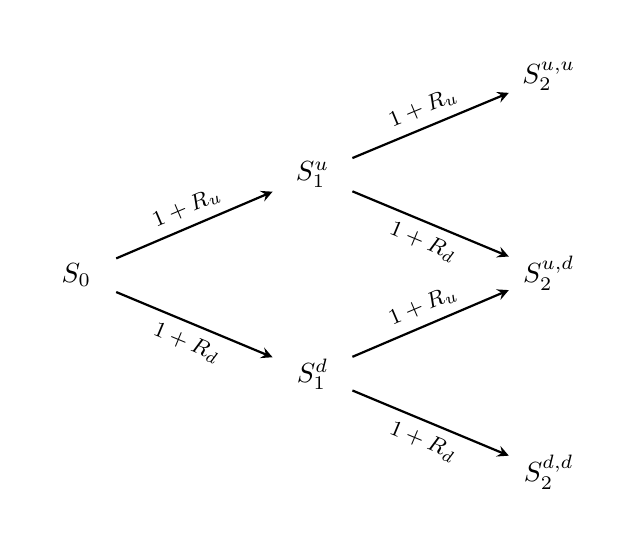
\begin{tikzpicture}[>=stealth,sloped]
        \matrix (tree) [%
          matrix of nodes,
          minimum size=1cm,
          column sep=2.0cm,
          row sep=.25cm,
        ]
        {
                &           & $S_2^{u,u}$   \\
                & $S_1^u$   &               \\
          $S_0$ &           & $S_2^{u,d}$   \\
                & $S_1^d$   &               \\
                &           & $S_2^{d,d}$   \\
        };
        \draw[->, thick] (tree-3-1) -- (tree-2-2) node [midway,above] {\footnotesize{$1 + R_u$}};
        \draw[->, thick] (tree-3-1) -- (tree-4-2) node [midway,below] {\footnotesize{$1 + R_d$}};
        \draw[->, thick] (tree-2-2) -- (tree-1-3) node [midway,above] {\footnotesize{$1 + R_u$}};
        \draw[->, thick] (tree-2-2) -- (tree-3-3) node [midway,below] {\footnotesize{$1 + R_d$}};
        \draw[->, thick] (tree-4-2) -- (tree-3-3) node [midway,above] {\footnotesize{$1 + R_u$}};
        \draw[->, thick] (tree-4-2) -- (tree-5-3) node [midway,below] {\footnotesize{$1 + R_d$}};
      \end{tikzpicture}
    \caption{A graphical representation of the 2-step binomial model.}
    \label{fig:2_step_binomial_model}
\end{figure}

\subsection{Model Setup}
Consider a model where only two assets are traded: A bond and a risky asset.
The bond satisfies that
\begin{align}
    B_t = (1+r), \quad t = 0,1, \ldots, T.
\end{align}
The price process $(S_t)_{t = 0,1, \ldots, T}$ satisfies that $S_0 > 0$ (non-random) and
\begin{align}
    S_t = S_{t - 1} (1 + K_s(t)), \quad t = 1, \ldots, T.
\end{align}
The returns are independent and identically distributed with
\begin{align}
    K_s(t) =
    \begin{cases}
        R_u &\text{with probability } p; \\
        R_d &\text{with probability } 1-p,
    \end{cases}
\end{align}
with the relation
\begin{align}
    R_d < R_u.
\end{align}

\subsection{Market Information}
I am considering the multi-step financial market
\begin{align}
    \mathfrak{M} = \left\{
        (\Omega, \mathscr{F}, \mathbb{P}),
        P = \left(
            B_t, S_t^{(1)}, S_t^{(2)}, \ldots, S_t^{(d)}
        \right)_{t = 0,1, \ldots, T}
    \right\}.
\end{align}
In order to further explain how information flows in the market i need to be more specific about the definition of the probability space.
I will start by letting
\begin{align}
    \Omega = \left\{
        \left(
            \omega^{(1)}, \omega^{(2)}, \ldots, \omega^{(T)}
        \right)
        \, : \,
        \omega^{(t)} \in \{u,d\}, \, t = 1, 2, \ldots, T
    \right\}.
\end{align}
Take for example the two-step binomial model, that is $T = 2$.
The vector $(d,u)$ represent the event in which the price went down in the first period and then up in the second period.

I will consider all possible events, which means that the $\sigma$-algebra in this case is
\begin{align}
    \mathscr{F} = 2^{\Omega}. \quad \text{(The power set)}
\end{align}
Using this set-up the return process can be written as
\begin{align}
    K_s(t)(\omega^{(1)}, \omega^{(2)}, \ldots, \omega^{(T)}) =
    \begin{cases}
        R_u & \text{if } \omega^{(t)} = u; \\
        R_d & \text{if } \omega^{(t)} = d. 
    \end{cases}
\end{align}
To ensure that the returns are independent and can go up and down with probability $p$ and $(1-p)$ respectively, i let
\begin{align}
    \mathbb{P}\left(
        \left\{
            \omega^{(1)}, \omega^{(2)}, \ldots, \omega^{(d)}
        \right\}
    \right) =
    p^k(1 - p)^{T-k},
\end{align}
where
\begin{align}
    k = \text{number of $u$'s in } \left(\omega^{(1)}, \omega^{(2)}, \ldots, \omega^{(d)}\right). 
\end{align}

As an example lets consider the two-step binomial model, that is $T = 2$ and we have that
\begin{align}
    \Omega = \left\{ uu, ud, du, dd \right\},
\end{align}
using the notational convention that
\begin{align}
    \left(
        \omega^{(1)}, \omega^{(2)}
    \right)
    =
    \omega^{(1)}\omega^{(2)}.
\end{align}
At time $t = 0$ no information is available but as time goes by, the price movements reveal information about future outcomes.
Say for example that at time $t = 1$ the price went down, the future outcomes are restricted to the set
\begin{align}
    B_d := \left\{ du, dd \right\},
\end{align}
as the the events $(uu)$ and $(ud)$ are no longer possible.

The aforementioned set is related to the information generated by the return process.
Consider the $\sigma$-field generated by a random variable, which is given by
\begin{align}
    \sigma(X) = \left\{
        X^{-1}(A) \, : \, A \in \mathscr{B}(\mathbb{R}).
    \right\}
\end{align}
Recall that for $t = 1,2$
\begin{align}
    K_S(t)\left(
        \omega^{(1)}, \omega^{(2)}
    \right) = 
    \begin{cases}
        R_u &\text{if } \omega^{(t)} = u; \\
        R_d &\text{if } \omega^{(t)} = d.
    \end{cases}
\end{align}
This tells me that, in the event that $K_S(1) = R_d$ it follows that
\begin{align}
    \left\{
        \left(
            \omega^{(1)}, \omega^{(2)}
        \right)
        \, : \,
        K_S(1) = R_d
    \right\} =
    \left\{
        du, dd 
    \right\} = B_d.
\end{align}
On the other hand if $K_S(1) = R_u$ it follows that
\begin{align}
    \left\{
        \left(
            \omega^{(1)}, \omega^{(2)}
        \right)
        \, : \,
        K_S(1) = R_u
    \right\} =
    \left\{
        uu, ud 
    \right\} = B_u.
\end{align}
Therefore
\begin{align}
    B_u, B_d \subseteq \sigma\left(K_S(1)\right).
\end{align}
It is in fact so, that because $K_S(1)$ only takes two values
\begin{align}
    \sigma(K_S(1)) = \left\{B_u, B_d, \Omega, \emptyset\right\}.
\end{align}

At the end of the trading period, in this case $t = T = 2$, the outcome of the price movements are known and stored in
\begin{align}
    \mathscr{F} = \sigma\left(K_S(1), K_S(2)\right).
\end{align}
Furthermore there has been constructed a family of sub-$\sigma$-algebras of $\mathscr{F}$;
\begin{align}
    \mathscr{F}_1 &= \sigma(K_S(1)) = \left\{B_u, B_d, \Omega, \emptyset\right\}. \\
    \mathscr{F}_2 &= \sigma(K_S(1), K_S(2)) = \mathscr{F}.
\end{align}
Note that by construction, $\mathscr{F}$ contains the whole information available on the price movements up until time $t$.
Mathematically this means that the price process $S_t$ is adapted to $\mathscr{F}$;
\begin{align}
    \sigma(S_t) \subseteq \mathscr{F}_t, \quad  t = 0,1,2 \text{ where } \mathscr{F}_0 = \left\{ \Omega, \emptyset \right\},
\end{align}
and moreover
\begin{align}
    \mathscr{F}_{t - 1} \subseteq \mathscr{F}_t, \quad t = 1,2.
\end{align}
A collection of sub-$\sigma$-algebras satisfying the previous relation is called a filtration.
A formal defintion is now given.
\begin{definition}[Filtrations and Adapted Process]
    Fix a probability space $(\Omega, \mathscr{F}, \mathbb{R})$.
    A collection of $\sigma$-algebras $\mathbb{F} = \left(\mathscr{F}_t\right)_{t = 0,1,\ldots,T}$ is called a filtration if for all $1 \leq t \leq T,$
    \begin{align}
        \mathscr{F}_{t - 1} \subseteq \mathscr{F}_{t} \subseteq \mathscr{F}.
    \end{align}
    The quadruplet
    \begin{align}
        (\Omega, \mathscr{F}, \left(\mathscr{F}_t\right)_{0 \leq t \leq T}, \mathbb{P}),
    \end{align}
    is termed a filtered probability space.
    
    Furthermore, a stochastic process $(X_t)_{0 \leq t \leq T}$ is said to be adapted to a filtration $\mathbb{F}$ if
    \begin{align}
        \sigma(X_t) \subseteq \mathscr{F}_t, \quad \forall 0 \leq t \leq T.
    \end{align}
\end{definition}

I am now able to give a formal definition of a financial market with information.
\begin{definition}[Financial Markets with Information]
    Fix $T, d \in \mathbb{N}$.
    A finite-horizon financial market with information is the pair
    \begin{align}
        \mathfrak{M} =
        \left\{
            \left(
                \Omega, 
                \mathscr{F}, 
                \left(
                    \mathscr{F}
                \right)_{0 \leq t \leq T},
                \mathbb{P}
            \right),
            P =
            \left(
                B_t,
                S_t^{(1)},
                \ldots,
                S_t^{(d)}
            \right)_{0 \leq t \leq T}
        \right\},
    \end{align}
    consisting of
    \begin{enumerate}
        \item A filtered probability space 
        $\left(
            \Omega, 
            \mathscr{F}, 
            \left(
                \mathscr{F}
            \right)_{0 \leq t \leq T},
            \mathbb{P}
        \right)$
        \item $P_t$ is adapted.
        \item $S^{(j)}$ is the price process of the $j$'th asset traded in the market
        \item B is a numéraire (e.g. a bond), i.e.
        \begin{align}
            \mathbb{P}(B_t > 0) = 1, 0 \leq t \leq T.
        \end{align}
    \end{enumerate}
\end{definition}

\subsection{Absence of Arbitrage}
An arbitrage is understood as a way to generate positive wealth with zero investment and zero risk.
In the one-step binomial model it is only allowed to allocate wealth ones, namely at time $t = 0$.
Returns are then measured at time $t = T = 1$.

In the multi-step binomial model agents will redesign their strategies based on the available information.
In order to create an arbitrage the portfolio need to be updated every time the price changes.
Therefore, instead of considering a single portfolio, an arbitrage now consists of a collection of portfolios $\left(\Theta_t\right)_{0 \leq t \leq T}$.
I will now give a formal definition of a portfolio and a strategy.
\begin{definition}[Portfolio and Strategy]
    A portfolio in $\mathfrak{M}$ is a $(d + 1)$-dimensional vector $\Theta_t = \left(\varphi_t, \theta_t^{(1)}, \ldots, \theta_t^{(d)}\right)$, in which
    \begin{align}
        \Theta_t^{(j)} = \text{ Number of shares of the $j$'th asset held between time $t - 1$ and $t$.}
    \end{align}
    The collection $\Theta = \left(\Theta_t\right)_{0 \leq t \leq T}$, with the convention that $\Theta_0 = \Theta_1$ is termed a strategy.
    
    The wealth process associated to $\Theta = \left(\Theta_t\right)_{0\leq t \leq T}$ is defined and denoted by
    \begin{align}
        V_t^\Theta :&= \varphi_tB_t + \sum_{j = 1}^d\theta_t^{(j)}S_t^{(j)} = \Theta_t \cdot P_t, \quad 0 \leq t \leq T \\
        \Rightarrow V_0^\Theta &= \varphi_0B_0 + \sum_{j = 1}^d\theta_0^{(j)}S_0^{(j)} = \varphi_1B_0 + \sum_{j = 1}^d\theta_1^{(j)}S_0^{(j)} 
    \end{align} 
\end{definition}
The arbitrage approach from the one-step binomial model can not be used when considering the multi-step binomial model as many strategies that from an intuitive point of view should not be thought of as an arbitrage, will be believed to be an arbitrage.
Consider for example the following situation
\begin{enumerate}
    \item Injection of capital at $t \geq 1$.
    \item Priviliged information.
    \item Unilimited credit.
\end{enumerate}
I therefore introduce the notion of an admissible strategy.
\begin{definition}[Admissible Strategy]
    Let $\Theta = \left(\varphi_t, \theta_t^{(1)}, \ldots, \theta_t^{(d)}\right)_{0 \leq t \leq T}$ be strategy on the market
    \begin{align}
        \mathfrak{M} =
        \left\{
            \left(
                \Omega, 
                \mathscr{F}, 
                \left(
                    \mathscr{F}
                \right)_{0 \leq t \leq T},
                \mathbb{P}
            \right),
            P =
            \left(
                B_t,
                S_t^{(1)},
                \ldots,
                S_t^{(d)}
            \right)_{0 \leq t \leq T}
        \right\}.
    \end{align}
    I will say that $\Theta$ is admissible if:
    \begin{enumerate}
        \item \textbf{It is self-financed}: It only requires initial capital.
        I will say that $\Theta$ is self financed if
        \begin{align}
            V_t^{\Theta} = \varphi_{t+1}B_t + \sum_{j=1}^d \theta_{t+1}^{(j)}S_t^{(j)}, \quad 0 \leq t \leq T-1. 
        \end{align}
        \item \textbf{Non-anticipative}: It is build up only on current information.
        I will say that $\Theta$ is non-anticipative or predictable if $\Theta_{t+1}$ depends only on the information at time $t$, that is $\Theta_{t+1}$ is $\mathscr{F}_t$-measurable.
        \item \textbf{It has a limited credit line}: There is a non-random constant $C > 0$, such that
        \begin{align}
            V_t^{\Theta} \geq -C, \ \forall \, 0 \leq t \leq T.
        \end{align}
    \end{enumerate}
\end{definition}
With this definition now in place i am able to define the concept of arbitrage in the multi-step binomial model
\begin{definition}[Arbitrage]
    Consider the market
    \begin{align}
        \mathfrak{M} =
        \left\{
            \left(
                \Omega, 
                \mathscr{F}, 
                \left(
                    \mathscr{F}
                \right)_{0 \leq t \leq T},
                \mathbb{P}
            \right),
            P =
            \left(
                B_t,
                S_t^{(1)},
                \ldots,
                S_t^{(d)}
            \right)_{0 \leq t \leq T}
        \right\}.
    \end{align}
    An admissible strategy $\Theta = \left(\varphi_t, \theta_t^{(1)}, \ldots, \theta_t^{(d)}\right)_{0 \leq t \leq T}$ is said to be an arbitrage if:
    \begin{enumerate}
        \item It has zero initial capital:
        \begin{align}
            V_0^\Theta = \varphi_0B_0 + \sum_{j = 1}^d\theta_0^{(j)} \cdot S_0^{(j)} = 0.
        \end{align}
        \item At time $t = T$, i am out of debts with 100\% certainty: Almost surely
        \begin{align}
            V_T^\Theta = \varphi_T B_T + \sum_{j = 1}^d\theta_T^{(j)} \cdot S_T^{(j)} \geq 0.
        \end{align}
        \item I have a chance to make a profit:
        \begin{align}
            \mathbb{P}
            \left(
                \varphi_TB_T + \sum_{j = 1}^d \theta_T^{(j)} \cdot S_T^{(j)} > 0
            \right) > 0.
        \end{align}
    \end{enumerate}
\end{definition}

\subsection{Risk-Neutral Measure}
To begin this section i will define the notion of a martingale.
Fix a filtered probability space
\begin{align}
    \left(
        \Omega, 
        \mathscr{F}, 
        \left(
            \mathscr{F}
        \right)_{0 \leq t \leq T},
        \mathbb{P}
    \right).
\end{align}
Recall that this means that $(\Omega, \mathscr{F}, (\mathscr{F}_t)_{0 \leq t \leq T}, \mathbb{P})$ is a probability space and $(\mathscr{F}_t)_{0 \leq t \leq T}$ is a filtration, i.e. a nested collection of sub-$\sigma$-algebras of $\mathscr{F}$: In symbols
\begin{align}
    \mathscr{F}_{t-1} \subseteq \mathscr{F}_t \subseteq \mathscr{F}, \quad \forall \, 1 \leq t \leq T. 
\end{align}
We are given a discrete time stochastic process
\begin{align}
    X = (X_t)_{0 \leq t \leq T}. 
\end{align}
Under this framework i give the definition of a martingale.
\begin{definition}[Martingale]\label{def:martingale}
    The collection $\{ (X_t, \mathscr{F}_t): t = 0,1, \ldots, T \}$ is said to be a martingale if
    \begin{enumerate}
        \item $X$ is adapted, i.e. $\sigma(X_t) \subseteq \mathscr{F}_t, \quad \forall \, 0 \leq t \leq T$.
        \item $X_t$ has finite first moment, that is $\mathbb{E}(|X_t|) < \infty$. 
        \item For all $0 \leq t \leq T-1$ we have that almost surely $\mathbb{E}(X_{t + 1} | \mathscr{F}_t) = X_t$. 
    \end{enumerate}
\end{definition}

\subsubsection{Binomial Model under Risk-Neutrality}
Consider the risk neutral multi-step binomial model: $B_0 = 1$, $S_0 > 0$ is a non-random constant and
\begin{align}
    B_t = (1 + r)^t; \quad S_t = S_{t-1}(1 + K_S(t)), \quad t = 1, \ldots, T. 
\end{align}
$(K_S(t))_{t = 1, \ldots, T}$ are i.i.d. with 
\begin{align}
    K_S(t) = 
    \begin{cases}
        R_u &\text{ with probability } q^* \\
        R_d &\text{ with probability } 1-q*
    \end{cases}
\end{align}
with the relation $R_d < r < R_u$ and
\begin{align}
    q^* = \frac{r - R_d}{R_u - R_d}; \quad R_d < r < R_u.
\end{align}
\task{Show derivation of $q^*$ (Thea)}
I will now show that the discounted price
\begin{align}
    X_t := \frac{S_t}{B_t}, \quad 0 \leq t \leq T, 
\end{align}
is a martingale under the filtration
\begin{align}
    \mathscr{F}_0 &= \{ \emptyset, \Omega\} \label{eq:information_at_time_0} \\
    \mathscr{F}_t &= \sigma(K_S(1), \ldots, K_S(t)), \quad 1 \leq t \leq T. \label{eq:information_at_time_1}  
\end{align}
In order to show this, i need to verify that the discounted price satisfies all three conditions in definition \ref{def:martingale} (\nameref{def:martingale})
\paragraph{Adapted}
\task{Get back to this lecture 6 part 5}

\paragraph{Finite First Moment}
\task{Get back to this lecture 6 part 5}

\paragraph{Martingale Property}
By definition
\begin{align}
    \mathbb{E}\left(X_{t + 1} | \mathscr{F}_t\right) &= \mathbb{E}\left(\frac{S_{t + 1}}{B_{t + 1}} \, \bigg| \, \mathscr{F}_t\right) \\
    &= \mathbb{E}\left(\frac{S_{t}(1 + K_S(t + 1))}{B_{t + 1}} \, \bigg| \, \mathscr{F}_t\right) \\
    &= \mathbb{E}\left(\frac{S_{t}(1 + K_S(t + 1))}{(1 + r)^{t + 1}} \, \bigg| \, \mathscr{F}_t\right) \\
    &= \mathbb{E}\left(\frac{S_{t}}{(1 + r)^{t + 1}}(1 + K_S(t + 1)) \, \bigg| \, \mathscr{F}_t\right) \\
    \text{{\footnotesize (By the Product Rule)}} &= \frac{S_{t}}{(1 + r)^{t + 1}}\mathbb{E}\left((1 + K_S(t + 1)) \, \bigg| \, \mathscr{F}_t\right) \\
    &= \frac{S_{t}}{(1 + r)^{t}}\frac{1}{(1 + r)}\mathbb{E}\left((1 + K_S(t + 1)) \, \bigg| \, \mathscr{F}_t\right) \\
    &= X_t\frac{1}{(1 + r)}\mathbb{E}\left((1 + K_S(t + 1)) \, \bigg| \, \mathscr{F}_t\right).
\end{align}
I am now left to show that
\begin{align}
    \mathbb{E}\left((1 + K_S(t + 1) \, \bigg| \, \mathscr{F}_t\right) = 1,
\end{align}
to do this i will use the independence of the returns but let me start by considering $t = 0$.
In this case
\begin{align}
    \mathbb{E}\left((1 + K_S(1)\,|\,\mathscr{F}_0\right) &= \mathbb{E}\left((1 + K_S(1)\,|\,\left\{\emptyset, \Omega\right\}\right) \\
    \text{{\footnotesize (Conditioning on the trivial $\sigma$-algebra)}} &= \mathbb{E}\left((1 + K_S(1)\right) \\
    \text{{\footnotesize (From Risk-Neutrality)}}&= (1 + r).
\end{align}
Let me now consider the case when $t \geq 1$
\begin{align}
    \mathbb{E}\left((1 + K_S(t + 1)\,|\,\mathscr{F}_t\right) &= \mathbb{E}\left((1 + K_S(t + 1)\,|\,K_S(1),\ldots,K_S(t)\right) \\
    \text{{\footnotesize (Indepence prop. of the cond. expectation)}} &= \mathbb{E}\left((1 + K_S(1)\right) \\
    &= (1 + r).
\end{align}

\newpage

\section{The First Fundamental Theorem of Asset Pricing}
\textit{Focus on explaining the hypothesis in the theorem (martingale measure, admissible strategies, arbitrage, etc.) and its applications to the pricing of financial derivatives.}

\subsection{The Theorem}
The Fundamental theorem of asset pricing gives necessary and sufficient conditions for the absence of arbitrage in the market with information, given by
\begin{align}\label{eq:market_with_information}
    \mathfrak{M} =
    \left\{
        \left(
            \Omega, 
            \mathscr{F}, 
            \left(
                \mathscr{F}_t
            \right)_{0 \leq t \leq T},
            \mathbb{P}
        \right),
        P =
        \left(
            B_t,
            S_t^{(1)},
            \ldots,
            S_t^{(d)}
        \right)_{0 \leq t \leq T}
    \right\}.
\end{align}

\begin{theorem}[FFTAP]\label{th:fftap}
    The market given by \eqref{eq:market_with_information} is arbitrage free if and only if there is a martingale measure. 
\end{theorem}

\subsection{Explaining the Hypothesis}

To understand the hypothesis presented in the theorem lets first remember the concept of an admissible strategy.
\begin{definition}[Admissible Strategy]
    Let $\Theta = \left(\varphi_t, \theta_t^{(1)}, \ldots, \theta_t^{(d)}\right)_{0 \leq t \leq T}$ be strategy on the market
    \begin{align}
        \mathfrak{M} =
        \left\{
            \left(
                \Omega, 
                \mathscr{F}, 
                \left(
                    \mathscr{F}_t
                \right)_{0 \leq t \leq T},
                \mathbb{P}
            \right),
            P =
            \left(
                B_t,
                S_t^{(1)},
                \ldots,
                S_t^{(d)}
            \right)_{0 \leq t \leq T}
        \right\}.
    \end{align}
    I will say that $\Theta$ is admissible if:
    \begin{enumerate}
        \item \textbf{It is self-financed}: It only requires initial capital.
        I will say that $\Theta$ is self financed if
        \begin{align}
            V_t^{\Theta} = \varphi_{t+1}B_t + \sum_{j=1}^d \theta_{t+1}^{(j)}S_t^{(j)}, \quad 0 \leq t \leq T-1. 
        \end{align}
        \item \textbf{Non-anticipative}: It is build up only on current information.
        I will say that $\Theta$ is non-anticipative or predictable if $\Theta_{t+1}$ depends only on the information at time $t$, that is $\Theta_{t+1}$ is $\mathscr{F}_t$-measurable.
        \item \textbf{It has a limited credit line}: There is a non-random constant $C > 0$, such that
        \begin{align}
            V_t^{\Theta} \geq -C, \ \forall \, 0 \leq t \leq T.
        \end{align}
    \end{enumerate}
\end{definition}
Next let me recall the notion of arbitrage.
\begin{definition}[Arbitrage]
    Consider the market
    \begin{align}
        \mathfrak{M} =
        \left\{
            \left(
                \Omega, 
                \mathscr{F}, 
                \left(
                    \mathscr{F}
                \right)_{0 \leq t \leq T},
                \mathbb{P}
            \right),
            P =
            \left(
                B_t,
                S_t^{(1)},
                \ldots,
                S_t^{(d)}
            \right)_{0 \leq t \leq T}
        \right\}.
    \end{align}
    An admissible strategy $\Theta = \left(\varphi_t, \theta_t^{(1)}, \ldots, \theta_t^{(d)}\right)_{0 \leq t \leq T}$ is said to be an arbitrage if:
    \begin{enumerate}
        \item It has zero initial capital:
        \begin{align}
            V_0^\Theta = \varphi_0B_0 + \sum_{j = 1}^d\theta_0^{(j)} \cdot S_0^{(j)} = 0.
        \end{align}
        \item At time $t = T$, i am out of debts with 100 \% certainty: Almost surely
        \begin{align}
            V_T^\Theta = \varphi_T B_T + \sum_{j = 1}^d\theta_T^{(j)} \cdot S_T^{(j)} \geq 0.
        \end{align}
        \item I have a chance to make a profit:
        \begin{align}
            \mathbb{P}
            \left(
                \varphi_TB_T + \sum_{j = 1}^d \theta_T^{(j)} \cdot S_T^{(j)} > 0
            \right) > 0.
        \end{align}
    \end{enumerate}
\end{definition}
In defining arbitrage i used the term admissible strategy, this will be repeated here.

Lastly i will define a martingale measure.
\begin{definition}[Martingale Measure]
    %Let 
    %\begin{align}
    %    \mathfrak{M} = \{ (\Omega, \mathscr{F}, (\mathscr{F}_t)_{0 \leq t \leq T}%, \mathbb{P}), P = (B_t, S_t^{(1)}, \ldots, S_t^{(d)})_{0 \leq t \leq T} \}
    %\end{align}
    %be the market. 
    Let $\mathbb{Q}$ be probability measure on $(\Omega, \mathscr{F})$, that is there are $0 < q^*_i < 1, i = 1, \ldots, N$ such that $\sum_{i=1}^N q^*_i = 1$ and 
    \begin{align}
        \mathbb{Q}(\{ \omega_i \}) = q^*_i \quad \text{for } i = 1, \ldots, N. 
    \end{align}
    We will say that $\mathbb{Q}$ is a martingale measure if under $\mathbb{Q}$ the discounted price $(\Tilde{P}_j^{(j)})_{0 \leq t \leq T}$ is a martingale w.r.t $(\mathscr{F}_t)_{0 \leq t \leq T}$, for every $j = 1,2, \ldots, d+1$.
\end{definition}

\subsection{Risk-Neutral and Martingale Measures}
In the binomial model $q^*$ plays two roles
\begin{enumerate}
    \item It transform the real-world probabilities (the one observed in the market) ($p$, $1-p$) satisfying that
    \begin{align}
        K_S(t) =
        \begin{cases}
            R_u & \text{with probability } p; \\
            R_d & \text{with probability } 1 - p,            
        \end{cases}
    \end{align}
    into a risk-neutral world in which the ``new'' distribution for the returns
    \begin{align}
        K_S(t) =
        \begin{cases}
            R_u & \text{with probability } q^*; \\
            R_d & \text{with probability } 1 - q^*,            
        \end{cases}
    \end{align}
    is such that
    \begin{align}
        \mathbb{E}_*(K_S(t)) = r, \quad t = 1,2,\ldots,T.
    \end{align}
    \item It transforms the discounted prices into a martingale.
\end{enumerate}
In this model the two are actually equivalent.
Consider the martingale property
\begin{align}
    \mathbb{E}_*\left( \frac{S_{t + 1}^{(j)}}{B_{t + 1}} \, \bigg| \, \mathscr{F}_t \right) &= \frac{S_{t}^{(j)}}{B_{t}} \\
    \frac{1}{B_{t + 1}}\mathbb{E}_*\left( S_{t + 1}^{(j)} \, \bigg| \, \mathscr{F}_t \right) &= \frac{S_{t}^{(j)}}{B_{t}} \\
    \frac{1}{S_{t}^{(j)}}\mathbb{E}_*\left( S_{t + 1}^{(j)} \, \bigg| \, \mathscr{F}_t \right) &= \frac{B_{t + 1}}{B_{t}} \\
    \mathbb{E}_*\left( \frac{S_{t + 1}^{(j)}}{S_{t}^{(j)}} \, \bigg| \, \mathscr{F}_t \right) &= \frac{B_{t + 1}}{B_{t}},
\intertext{subtracting 1 from both sides i get}
    \mathbb{E}_*\left( \frac{S_{t + 1}^{(j)}}{S_{t}^{(j)}} - 1 \, \bigg| \, \mathscr{F}_t \right) &= \frac{B_{t + 1}}{B_{t}} - 1,
\intertext{taking expectations gives}
    \mathbb{E}\left[\mathbb{E}_*\left( \frac{S_{t + 1}^{(j)}}{S_{t}^{(j)}} - 1 \, \bigg| \, \mathscr{F}_t \right)\right] &= \mathbb{E}\left[\frac{B_{t + 1}}{B_{t}} - 1\right] \\
    \mathbb{E}_*\left( \frac{S_{t + 1}^{(j)}}{S_{t}^{(j)}} - 1 \right) &= \frac{B_{t + 1}}{B_{t}} - 1 \\
    \mathbb{E}_*\left( K_S(t + 1) \right) &= K_B(t + 1).
\end{align}
This is exactly the definition of risk-neutral probabilities.

\task{Add application to the pricing of financial derivaties.}

\newpage

\section{Pricing in the Binomial Model}
\textit{Explain what is the typical methodology for pricing derivatives and how such a methodology works in the Binomial model. Remember to include an example (e.g. the price of call-option).}

\subsection{Methodology for Pricing}
I will start by outlining the methodology used for pricing derivatives in the binomial model.
\begin{enumerate}
    \item \textbf{Define a model for the prices}: Specify the dynamics for
    \begin{align}
        P = 
        \left(
            B_t, S_t^{(1)}, \ldots, S_t^{(d)}
        \right)_{0 \leq t \leq T},
    \end{align}
    i.e. describe how the distribution, evolution and behavior of the prices should be\dots according to some empirical facts observed in the data.
    \item \textbf{Indicate a set of information}: Determine what information is available at each point in time, i.e. specify $\left(\mathscr{F}_t\right)_{0 \leq t \leq T}$.
    \item \textbf{Check for arbitrage opportunities}: Establish under which circumstances the proprosed model does not admit an arbitrage, i.e. by the First Fundamental Theorem of Asset Pricing find a martingale measure $\mathbb{Q}$ for the model.
    \item \textbf{Dynamics in the risk-neutral world}: Investigate what the distribution of the price process is under the martingale measure.
    This is necessary as the $\xi = \Phi(P_0, \dots, P_T)$ is a function of the prices.
    \item \textbf{Price the derivative}: Compute the prices of the derivative by
    \begin{align}
        \xi_t := \mathbb{E}_*\left(\frac{B_t}{B_T}\xi \, \bigg| \, \mathscr{F}_t\right)
    \end{align}
\end{enumerate}

\subsection{Define a model for the prices}
In this part I will consider multi-step binomial model. 
Only a bond and a risky asset are traded. 
The bond price is given by
\begin{align}
    B_t = (1+r)^t, \quad t= 0,1, \ldots, T.
\end{align}
The price of the risky asset is given by $S_0 > 0$ (non-random) and 
\begin{align}
    S_t = S_{t-1} (1 + K_S(t)), \quad t = 1, \ldots, T
\end{align}
where 
\begin{align}
    K_S(t) = 
    \begin{cases} 
        R_u & \text{ with probability } p;\\ 
        R_d & \text{ with probability } 1 - p,
    \end{cases}
\end{align}
with the relation $R_d < R_u$. 

\subsection{Indicate a set of information}
I assume that the market movements are exclusively determined by the behavior of the returns, that is
\begin{align}
    \mathscr{F}_0 = \{\emptyset, \Omega\}, \ \mathscr{F}_t = \sigma(K_S(1), \ldots, K_S(t)), \quad 1 \leq t \leq T. 
\end{align}

\subsection{Check for arbitrage opportunities}
The market does not admit an arbitrage if and only if
\begin{align}
    R_d < r < R_u. 
\end{align}
\task{Explain why}
In this situation a martingale measure exists: Under $\mathbb{Q}$ the returns are i.i.d. and satisfies that 
\begin{align}
    \mathbb{Q}(K_S(t) &= R_u) = q^*;\\
    \mathbb{Q}(K_S(t) &= R_d) = 1 - q^*. 
\end{align}
Where
\begin{align}
    q^* = \frac{r - R_d}{R_u - R_d}. 
\end{align}

\subsection{Dynamics in the risk-neutral world}
To find the distribution of prices under $\mathbb{Q}$ in the multistep binomial model, i present the following proposition. 
\begin{proposition}
    In the multi-step binomial model it holds that for all $t = 1, \ldots, T$
    \begin{align}
        S_t = S_0(1 + R_u)^{N_t}(1+R_d)^{t-N_t}
    \end{align}
    where $N_t$ is the number of times the price went up during $t$ periods and
    \begin{align}
        \mathbb{Q}(N_t = x) = \binom{t}{x}(q^*)^x(1-q)^{t-x}, x = 0, \ldots, t. 
    \end{align}
    In particular 
    \begin{align}
        \mathbb{Q} \Big[S_t = S_0(1+R_u)^x(1+R_d)^{t-x}\Big] = \binom{t}{x} (q^*)^x(1-q^*)^{t-x},
    \end{align}
    for $x = 0, 1, \ldots, t$. 
\end{proposition}
\textbf{Remark:} $N_t$ represents the number of times that the price went up during the periods $1, 2, \ldots, t$. In particular, under the risk neutral measure
\begin{align}
    N_t \sim Bin(t, q^*)
\end{align}

\subsection{Pricing a Call Option}
Let us now find the inital price of a call option. 
Recall that such a contract gives the owner the right but not the obligation to buy an asset at a given value, say $C > 0$ at a predetermined point in time, say $T > 0$. 

The pay-off is then given by the random variable
\begin{align}
    \xi = \max\{ S_T - C, 0\} = (S_T - C)^+.
\end{align}
Independently of the model, we know by theorem \ref{th:fftap} (FFTAP) that the arbitrage free initial price of such an option is 
\begin{align}
    \xi_0 = \mathbb{E}_*\left( \frac{B_0}{B_T}(S_T - C)^+\right). 
\end{align}
In the multi-step binomial model we have
\begin{align}
    \xi_0 = \mathbb{E}_* \left( \frac{B_0}{B_T}(S_T - C)^+ \right) = \frac{1}{(1+r)^T} \mathbb{E}_* \left( (S_T-C)^+\right). 
\end{align}
Using that under the probability measure $\mathbb{Q}$ we have that for all $x = 0, \ldots, T$
\begin{align}
    p_T(x; q^*) &= \mathbb{Q}\left[ S_T := S_0(1+ R_u)^x(1+R_d)^{T-x}\right]\\
    &= \binom{T}{x}( q^* )^x(1-q^*)^{T-x}
\end{align}
it follows that 
\begin{align}
    \mathbb{E}_* \left( (S_T - C)^+ \right) = \sum_{x=0}^T \left( S_0(1+R_u)^x(1+R_d)^{T-x} - C \right)^+ p_T(x; q^*).
\end{align}
Observe that 
\begin{align}
    \left( S_0(1+R_u)^x(1+R_d)^{T-x} - C \right)^+ \neq 0
\end{align}
if and only if 
\begin{align}
     S_0(1+R_u)^x(1+R_d)^{T-x} > C. 
\end{align}
Let (with the convention that $\min\{ \emptyset \} = + \infty$)
\begin{align}
    x_0(S_0, R_u, R_d, T) = \min\{ 0 \leq x \leq T : S_0(1 + R_u)^x(1+R_d)^{T-x} > C\}. 
\end{align}
Then 
\begin{align}
    \mathbb{E}_*\left( (S_T - C)^+\right) &= \sum_{x=0}^T \left( S_0(1+R_u)^x(1 + R_d)^{T-x}  - C \right)^+ p_T(x; q^*)\\
    &= \sum_{x=x_0}^T \left( S_0(1+R_u)^x(1 + R_d)^{T-x}  - C \right)^+ p_T(x; q^*)\\
    &= S_0 \sum_{x=x_0}^T \left((1+R_u)^x(1 + R_d)^{T-x}  - C \right)^+ p_T(x; q^*)
    \\ &\qquad 
    - C \sum_{x=x_0}^T p_T (x; q^*). 
\end{align}
Since 
\begin{align}
    p_T(x; q^*) = \mathbb{Q} \left[ S_T = S_0(1 + R_u)^x(1+R_d)^{t-x} \right] = \binom{T}{x}(q^*)^x(1-q^*)^{T-x}
\end{align}
Then
\begin{align}
   (1+R_u)^x(1+R_d)^{T-x} p_T(x; q^*) &= (1+R_u)^x(1+R_d)^{T-x} \times \binom{T}{x} (q^*)^x(1-q^*)^{T-x}\\
&= \binom{T}{x} [(1 + R_u)q^*]^x \times [(1+R_d)(1-q^*)]^{T-x}
\end{align}
All in all this implies that the arbitrage free initial price of a call option in the multi step binomial model is given by the formula
\begin{align}\label{eq:crr}
    \xi_0 = \mathbb{E}_* \left( \frac{(S_T - C)^+}{(1+r)^T} \right) = S_0 \Psi_1(T, S_0, C, q^*) - \frac{C}{(1+r)^T} \Psi_2(T, S_0, C, q^*)
\end{align}
where 
\begin{align}
    \Psi_1 (T, S_0, C, q^*) &:= \sum_{x = x_0}^T \binom{T}{x} \left[ \frac{1 + R_u}{1+r} q^* \right]^x\left[ \frac{1+R_d}{1+r}(1 - q^*) \right]^{T-x}\\
    \Psi_2 (T, S_0, C, q^*) &:= \sum_{x = x_0}^T p_T(x; q^*)
\end{align}
in which 
\begin{align}
    x_0 = x_0(S_0, R_u, R_d, T) = min\{ 0 \leq x \leq T : S_0(1+R_u)^x(1+R_d)^{T-x} > C\}
\end{align}
The expression in \eqref{eq:crr} is known as the \textbf{Cox-Ross-Rubenstein} formula.

\subsection{Price function for simple derivatives}

\begin{theorem}[Price Function]\label{th:price_function}
    Within the framework of the multi-step binomial model, let $\xi$ be a simple derivative, that is $\xi = \varphi(S_T)$. 
    Put
    \begin{align}
        F(t,y) := \frac{1}{(1+r)^{T-t}} \mathbb{E}_* \{ \varphi (S_{T-t}^y) \}, \quad y \geq 0, \ 0 \leq t \leq T, 
    \end{align}
    where $(S_t^y)_{0 \leq t \leq T}$ is a process satisfying that $S_0^y = y$ and 
    \begin{align}
        S_t^y = S_{t-1}^y(1 + K_S(t)), t = 1, \ldots, T. 
    \end{align}
    Then, almost surely
    \begin{align}
        F(t, S_t) = \frac{1}{(1+r)^{T-t}} \mathbb{E}_* (\varphi(S_T) | \mathscr{F}_t), 0 \leq t \leq T. 
    \end{align}
    In other words the arbitrage free price of the simple derivative $\xi = \varphi(S_T)$ at time $0 \leq t \leq T$ is given by $F(t, S_t)$. 
\end{theorem}

\textbf{Remark: } The function $F$ is known as the price function associated to the pay-off function $\varphi$. 

\textbf{Interpretation: } The function $F(t,y)$ can be thought as the initial price of a simple derivative with maturity time $T-t$ and pay-off function $\varphi$ under the circumstances that the initial price of the risky asset is $y \geq 0$. 

\subsection{General Price of a Call option in the Binomial Model}
According to the previous theorem the price of a call option in the multi step binomial model at time $t = 0,1, \ldots, T$ is given by 
\begin{align}
    \xi_t = F(t, S_t) = \frac{1}{(1+r)^{T-t}} \mathbb{E}_* \left( (S_T - C)^+ | \mathscr{F}_t \right)
\end{align}
where 
\begin{align}
    F(t,y) = \mathbb{E}_* \left[ \frac{(S_{T-t}^y - C)^+}{(1+r)^{T-t}} \right], y \geq 0, 0 \leq t \leq T
\end{align}
in which $(S_t^y)_{0 \leq t \leq T}$ is a process satisfying that $S_0^y = y$ and 
\begin{align}
    S_t^y = S_{t-1}^y(1 + K_S(t)), t = 1, \ldots, T. 
\end{align}
The Cox-Ross-Rubunstein formula dictates that 
\begin{align}
    F(t, S_0) &= \mathbb{E}_* \left(  \frac{(S_{T-t} - C)^+}{(1+r)^{T-t}} \right)\\
    &= S_0 \Psi_1 (T-t, S_0, C, q^*) - \frac{C}{(1+r)^{T_0}} \Psi_2(T-t, S_0, C, q^*).
\end{align}

Replacing $S_0$ by $y$ the Cox-Ross-Rubenstein formula we get that 
\begin{align}
    F(t, y) = y \Psi_1 (T-t, y, C, q^*) - \frac{C}{(1+r)^{T-t}}\Psi_2(T-t, y, C, q^*). 
\end{align}
Hence the price call option in the multi-step binomial model is 
\begin{align}
    \xi_t = F(t, S_t) = S_t \Psi_1(T-t, S_t,C, q^*) - \frac{C}{(1+r)^{T-t}} \Psi_2(T-t, S_t, C, q^*).
\end{align}

\newpage

\section{The Second Fundamental Theorem of Asset Pricing}
\textit{Focus on explaining the hypothesis in the theorem (martingale measure, admissible strategies, arbitrage, completeness, etc.) and its consequences on the pricing of financial derivatives. You can, in particular, show that the Binomial Model is complete while the Trinomial Model is not.}

\subsection{Market}
The market with information is given
\begin{align*}
    \mathfrak{M} = \{ (\Omega, \mathscr{F}, (\mathscr{F}_t)_{0 \leq t \leq T}, \mathbb{P}), P = (B_t, S_t^{(1)}, \ldots, S_t^{(d)})_{0 \leq t \leq T} \}. 
\end{align*} 
The filtered probability space $(\Omega, \mathscr{F}, (\mathscr{F}_t)_{0 \leq t \leq T}, \mathbb{P})$ satisfies that 
\begin{enumerate}
    \item The sample space is finite and our $\sigma$-algebra is the power set: 
    \begin{align*}
       \Omega = \{ \omega_1, \ldots, \omega_N\}, \ N \in \mathbb{N}, \ \mathscr{F} = 2^{\Omega}.
    \end{align*}
    \item There are $0 < p_i < 1$ for $i = 1, \ldots, N$ such that 
    \begin{align*}
        \sum_{i=1}^N p_i &= 1\\
        \mathbb{P}(\{ \omega_i \}) &= p_i, \quad i = 1, \ldots, N
    \end{align*}
    \item The set of information satisfies that $\mathscr{F}_0 = \{ \emptyset, \Omega\}, \mathscr{F}_T = \mathscr{F}$, and 
    \begin{align*}
        \mathscr{F}_{t-1} \subseteq \mathscr{F}_t, \quad 1 \leq t \leq T-1. 
    \end{align*}
\end{enumerate}
We will assume that $B$ is deterministic, $B_0 = 1$ and $B_t > 0$, $\forall \ 1 \leq t \leq T$.

\subsection{The Theorem}
\begin{theorem}[Second Fundamental Theorem of Asset Pricing]
    Let the market 
    \begin{align*}
        \mathfrak{M} = \left\{ (\Omega, \mathscr{F}, (\mathscr{F}_t)_{0 \leq t \leq T}, \mathbb{P}), P = \left(B_t, S_t^{(1)}, \ldots, S_t^{(d)}\right)_{0 \leq t \leq T} \right\}. 
    \end{align*} 
    be as described. 
    Then $\mathfrak{M}$ is complete and arbitrage free if and only if there is a unique martingale measure.
\end{theorem}

\subsection{Definitions}
\begin{definition}[Martingale]
    The collection $\{ (X_t, \mathscr{F}_t): t = 0,1, \ldots, T \}$ is said to be a martingale if
    \begin{enumerate}
        \item $X$ is adapted, i.e. $\sigma(X_t) \subseteq \mathscr{F}_t, \quad \forall \, 0 \leq t \leq T$.
        \item $X_t$ has finite first moment, that is $\mathbb{E}(|X_t|) < \infty$. 
        \item For all $0 \leq t \leq T-1$ we have that almost surely $\mathbb{E}(X_{t + 1} | \mathscr{F}_t) = X_t$. 
    \end{enumerate}
\end{definition}
\begin{definition}[Martingale Measure]
    %Let 
    %\begin{align}
    %    \mathfrak{M} = \{ (\Omega, \mathscr{F}, (\mathscr{F}_t)_{0 \leq t \leq T}%, \mathbb{P}), P = (B_t, S_t^{(1)}, \ldots, S_t^{(d)})_{0 \leq t \leq T} \}
    %\end{align}
    %be the market. 
    Let $\mathbb{Q}$ be probability measure on $(\Omega, \mathscr{F})$, that is there are $0 < q^*_i < 1, i = 1, \ldots, N$ such that $\sum_{i=1}^N q^*_i = 1$ and 
    \begin{align}
        \mathbb{Q}(\{ \omega_i \}) = q^*_i \quad \text{for } i = 1, \ldots, N. 
    \end{align}
    We will say that $\mathbb{Q}$ is a martingale measure if under $\mathbb{Q}$ the discounted price $(\Tilde{P}_j^{(j)})_{0 \leq t \leq T}$ is a martingale w.r.t $(\mathscr{F}_t)_{0 \leq t \leq T}$, for every $j = 1,2, \ldots, d+1$.
\end{definition}
\begin{definition}[Admissible Strategy]
    Let $\Theta = \left(\varphi_t, \theta_t^{(1)}, \ldots, \theta_t^{(d)}\right)_{0 \leq t \leq T}$ be strategy on the market
    \begin{align}
        \mathfrak{M} =
        \left\{
            \left(
                \Omega, 
                \mathscr{F}, 
                \left(
                    \mathscr{F}
                \right)_{0 \leq t \leq T},
                \mathbb{P}
            \right),
            P =
            \left(
                B_t,
                S_t^{(1)},
                \ldots,
                S_t^{(d)}
            \right)_{0 \leq t \leq T}
        \right\}.
    \end{align}
    I will say that $\Theta$ is admissible if:
    \begin{enumerate}
        \item \textbf{It is self-financed}: It only requires initial capital.
        I will say that $\Theta$ is self financed if
        \begin{align}
            V_t^{\Theta} = \varphi_{t+1}B_t + \sum_{j=1}^d \theta_{t+1}^{(j)}S_t^{(j)}, \quad 0 \leq t \leq T-1. 
        \end{align}
        \item \textbf{Non-anticipative}: It is build up only on current information.
        I will say that $\Theta$ is non-anticipative or predictable if $\Theta_{t+1}$ depends only on the information at time $t$, that is $\Theta_{t+1}$ is $\mathscr{F}_t$-measurable.
        \item \textbf{It has a limited credit line}: There is a non-random constant $C > 0$, such that
        \begin{align}
            V_t^{\Theta} \geq -C, \ \forall \, 0 \leq t \leq T.
        \end{align}
    \end{enumerate}
\end{definition}
\begin{definition}[Arbitrage]
    Consider the market
    \begin{align}
        \mathfrak{M} =
        \left\{
            \left(
                \Omega, 
                \mathscr{F}, 
                \left(
                    \mathscr{F}_t
                \right)_{0 \leq t \leq T},
                \mathbb{P}
            \right),
            P =
            \left(
                B_t,
                S_t^{(1)},
                \ldots,
                S_t^{(d)}
            \right)_{0 \leq t \leq T}
        \right\}.
    \end{align}
    An admissible strategy $\Theta = \left(\varphi_t, \theta_t^{(1)}, \ldots, \theta_t^{(d)}\right)_{0 \leq t \leq T}$ is said to be an arbitrage if:
    \begin{enumerate}
        \item It has zero initial capital:
        \begin{align}
            V_0^\Theta = \varphi_0B_0 + \sum_{j = 1}^d\theta_0^{(j)} \cdot S_0^{(j)} = 0.
        \end{align}
        \item At time $t = T$, i am out of debts with 100 \% certainty: Almost surely
        \begin{align}
            V_T^\Theta = \varphi_T B_T + \sum_{j = 1}^d\theta_T^{(j)} \cdot S_T^{(j)} \geq 0.
        \end{align}
        \item I have a chance to make a profit:
        \begin{align}
            \mathbb{P}
            \left(
                \varphi_TB_T + \sum_{j = 1}^d \theta_T^{(j)} \cdot S_T^{(j)} > 0
            \right) > 0.
        \end{align}
    \end{enumerate}
\end{definition}
\begin{definition}[Complete Financial Market]
    The market is said to be complete if every European contingent claim $\xi$ (i.e. a random variable that depends on the information up to time $T$) can be replicated, that is, there exists an admissible strategy
    \begin{align}
        \Theta = \left(\varphi_t, \theta_t^{(1)}, \ldots, \theta_t^{(d)}\right)_{0 \leq t \leq T}
    \end{align}
    such that almost surely
    \begin{align}
        \xi = V_T^{\Theta} = \varphi B_T + \sum_{j = 1}^d \theta_T^{(j)}S_T^{(j)}.
    \end{align}
\end{definition}
This means that, if the market is arbitrage free and $\mathbb{P}\left(\xi > 0\right) > 0$, then necessarily
\begin{align}
    V_0^\Theta > 0.
\end{align}

\subsection{Remarks}
If the market is arbitrage free and complete, the we have a unique arbitrage-free price for any derivative with pay-off $\xi$ which is given by
\begin{align}
    \mathbb{E}_*\left(\frac{B_t}{B_T}\xi\,\bigg|\,\mathscr{F}_t\right).
\end{align}

\end{document}